\documentclass{beamer}
\setbeamertemplate{navigation symbols}{}
\setbeamertemplate{bibliography item}[text]

\usepackage{beamerthemeshadow}
\usepackage{amsmath}
\usepackage{amssymb}
\usepackage{graphicx}
\graphicspath{ {./images/} }
\begin{document}
\title{Convex Sets, Convex Hull}  
\author{Coman Florin-Alexandru}

\begin{frame}
\titlepage
\end{frame}

\begin{frame}\frametitle{Table of contents}\tableofcontents
\end{frame}

\section{Convex Sets}
\subsection{Introduction}
\begin{frame}{Convex Sets}
\begin{block}{Convex Sets}
Intuitively, if we think of $\mathbb{R}^2$ or $\mathbb{R}^3$, a convex set of vectors is a set that contains all the points of any line segment joining two points of the set.
\end{block}
\begin{exampleblock}{Examples}
\begin{figure}[h]
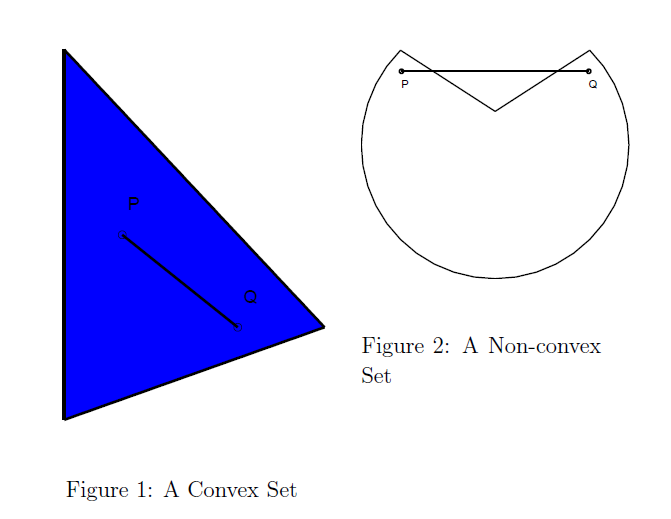
\includegraphics[width=4cm]{picture1}
\end{figure}
\end{exampleblock}
\end{frame}

\subsection{Convex Combinations}
\begin{frame}{Convex Sets}
\begin{block}{Convex Combinations - Definition}
Let $u, v \in V$. Then the set of all \textbf{convex combinations} of $u$ and $v$ is the set of points
\centerline{$\lbrace \omega_\lambda \in V : \omega_\lambda = (1 - \lambda) u + \lambda v, 0 \leq \lambda \leq 1 \rbrace$ \hspace{0.5cm} (1.1)}
\end{block}
\begin{exampleblock}{}
For example, in $\mathbb{R}^2$, this set is exactly the line segment joining the two points $u$ and $v$.
\end{exampleblock}
\end{frame}

\subsection{Definition}
\begin{frame}{Convex Sets}
\begin{block}{Definition}
Let $K \subset V$. Then the set $K$ is said to be \textbf{convex} provided that given two points $u, v \in K$ the set (1.1) is a subset of $K$.
\end{block}
\begin{exampleblock}{Example}
An interval $[a, b] \subset \mathbb{R}$ is a convex set. \\
To see this, let $c, d \in [a, b]$ and assume, without loss of generality, that $c < d$. Let $\lambda \in (0, 1)$. Then, \\
$a \leq c = (1 - \lambda) c + \lambda c < (1 - \lambda) c + \lambda d$ \\
\hspace{0.18cm} $\leq (1 - \lambda) d + \lambda d = d$ \\
\hspace{0.18cm} $\leq b.$
\end{exampleblock}
\end{frame}

\subsection{Properties}
\begin{frame}{Convex Sets}
\begin{block}{Proposition 1.1}
If $X$ is a convex set and $\beta \in \mathbb{R}$, the set $\beta X = \lbrace y : y = \beta x, x \in X \rbrace$ is convex.
\end{block}
\begin{block}{Proof}
\begin{figure}[h]
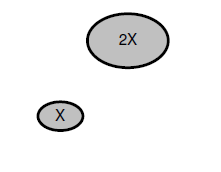
\includegraphics[width=4cm]{picture2}
\end{figure}
\end{block}
\end{frame}

\begin{frame}{Convex Sets}
\begin{block}{Proposition 1.2}
If $X$ and $Y$ are convex sets, then the set \\
$X + Y = \lbrace z : z = x + y, x \in X, y \in Y \rbrace$ is convex.
\end{block}
\begin{block}{Proof}
\begin{figure}[h]
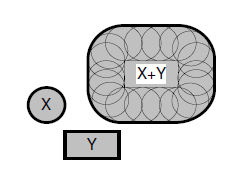
\includegraphics[width=4cm]{picture3}
\end{figure}
\end{block}
\end{frame}

\begin{frame}{Convex Sets}
\begin{block}{Proposition 1.3}
The intersection of any collection of convex sets is convex.
\end{block}
\begin{block}{Proof}
\begin{figure}[h]
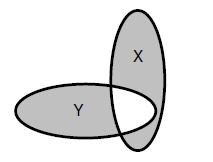
\includegraphics[width=4cm]{picture4}
\end{figure}
\end{block}
\end{frame}

\section{Convex Hull}
\subsection{Definition}
\begin{frame}{Convex Hull}
\begin{block}{Definition}
The \textbf{convex hull} of a set $C$ is the intersection of all convex sets which contain the set $C$. 
\end{block}
\end{frame}

\subsection{Example}
\begin{frame}{Convex Hull}
\begin{exampleblock}{Example}
\begin{figure}[h]
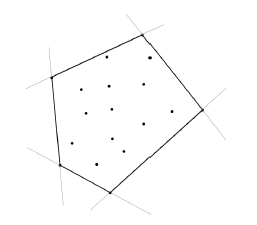
\includegraphics[width=4cm]{picture5}
\end{figure}
Representation of a convex set as the convex hull of a set of points.
\end{exampleblock}
\end{frame}

\section{Algorithms for Computing Planar Convex Hulls}
\subsection{The Jarvis March Algorithm}
\begin{frame}{Convex Hulls - Algorithms}
\begin{block}{The Jarvis March Algorithm}
\fontsize{6pt}{7.2}\selectfont
\texttt{jarvis(S) \\
   \hspace*{0.5cm}pointOnHull = leftmost point in S \\
   \hspace*{0.5cm}i = 0 \\
   \hspace*{0.5cm}repeat \\
      \hspace*{1cm}P[i] = pointOnHull \\
      \hspace*{1cm}endpoint = S[0]         /* initial endpoint for a candidate edge on the hull */ \\
 \hspace*{1cm}for j from 1 to |S| \\
         \hspace*{1.5cm}if (endpoint == pointOnHull) or (S[j] is on left of line from P[i] to endpoint) \\
            \hspace*{2cm}endpoint = S[j]   /* found greater left turn, update endpoint */ \\
      \hspace*{1cm}i = i+1 \\
      \hspace*{1cm}pointOnHull = endpoint \\
   \hspace*{0.5cm}until endpoint == P[0]      /* wrapped around to first hull point*/ }
\end{block}
\end{frame}

\subsection{The Andrew's Algorithm}
\begin{frame}{Convex Hulls - Algorithms}
\begin{block}{The Andrew's Algorithm}
\fontsize{6pt}{7.2}\selectfont
\texttt{Input: a list P of points in the plane. \\
Sort the points of P by x-coordinate (in case of a tie, sort by y-coordinate). \\
Initialize U and L as empty lists. \\
The lists will hold the vertices of upper and lower hulls respectively.}
\end{block}
\begin{block}{}
\fontsize{6pt}{7.2}\selectfont
\texttt{for i = 1, 2, ..., n: \\
    \hspace*{0.5cm}while L contains at least two points and the sequence of last two points of L and the\\
			\hspace*{1.5cm}point P[i] doesn't make a counter-clockwise turn:\\
        \hspace*{1cm}remove the last point from L \\
    \hspace*{0.5cm}append P[i] to L \\ 
for i = n, n-1, ..., 1: \\
    \hspace*{0.5cm}while U contains at least two points and the sequence of last two points of U and the\\
			\hspace*{1.5cm}point P[i] doesn't make a counter-clockwise turn: \\
        \hspace*{1cm}remove the last point from U \\
    \hspace*{0.5cm}append P[i] to U}
\end{block}
\begin{block}{}
\fontsize{6pt}{7.2}\selectfont
Remove the last point of each list (it's the same as the first point of the other list). \\
Concatenate L and U to obtain the convex hull of P. \\
Points in the result will be listed in counter-clockwise order.
\end{block}
\end{frame}

\subsection{The Chan's Algorithm}
\begin{frame}{Convex Hulls - Algorithms}
\begin{block}{FindHull($P$, $m$)}
\fontsize{6pt}{7.2}\selectfont
\texttt{Partition $P$ into n/m groups $P_i$\\
for i = 1 ... n/m: \\
	\hspace*{1cm} $\mathcal{H}_i$ = ConvexHull($P_i$) \\
Run Jarvis march on $\lbrace \mathcal{H}_i \rbrace$ for $m$ steps \\
if we get a complete hull then \\
	\hspace*{1cm} return success\\
else \\
	\hspace*{1cm} return fail}
\end{block}
\begin{block}{Chan's Algorithm}
\fontsize{6pt}{7.2}\selectfont
\texttt{i = 0 \\
while FindHull($P, 2^{2^i}$) fails \\
	\hspace*{1cm}i = i + 1}
\end{block}
\end{frame}

\subsection{Quickhull Algorithm}
\begin{frame}{Convex Hulls - Algorithms}
\begin{block}{Quickhull Algorithm}
\fontsize{9pt}{7.2}\selectfont
1. Find the points with minimum and maximum x coordinates, those are bound to be part of the convex hull. \\
2. Use the line formed by the two points to divide the set in two subsets of points, which will be processed recursively. \\
3. Determine the point, on one side of the line, with the maximum distance from the line. The two points found before along with this one form a triangle. \\
4. The points lying inside of that triangle cannot be part of the convex hull and can therefore be ignored in the next steps. \\
5. Repeat the previous two steps on the two lines formed by the triangle (not the initial line). \\
6. Keep on doing so on until no more points are left, the recursion has come to an end and the points selected constitute the convex hull. \\
\end{block}
\end{frame}

\subsection{Graham scan algorithm}
\begin{frame}{Convex Hulls - Algorithms}
\begin{block}{Graham scan algorithm I}
\fontsize{6pt}{7.2}\selectfont
\texttt{/* Three points are a counter-clockwise turn if ccw > 0, clockwise if ccw < 0, and collinear if ccw = 0 because ccw is a determinant that gives twice the signed  area of the triangle formed by p1, p2 and p3.*/ \\
function ccw(p1, p2, p3): \\
    \hspace*{1cm}return (p2.x - p1.x)*(p3.y - p1.y) - (p2.y - p1.y)*(p3.x - p1.x) \\ }
\end{block}
\end{frame}

\begin{frame}{Convex Hulls - Algorithms}
\begin{block}{Graham scan algorithm II}
\fontsize{6pt}{7.2}\selectfont
N  = number of points \\
points[N+1] = the array of points \\
swap points[1] with the point with the lowest y-coordinate sort points by polar angle with points[1] \\
/* We want points[0] to be a sentinel point that will stop the loop. */ \\
points[0] = points[N] \\
/* M will denote the number of points on the convex hull.  */ \\
M = 1 \\
for i = 2 to N: \\
    \hspace*{1cm}/* Find next valid point on convex hull. */ \\
    \hspace*{1cm}while ccw(points[M-1], points[M], points[i]) <= 0: \\
          \hspace*{1.5cm}if M > 1: \\
                  \hspace*{2cm}M -= 1 \\
          \hspace*{1.5cm}/* All points are collinear */ \\
          \hspace*{1.5cm}else if i == N: \\
                  \hspace*{2cm}break \\
          \hspace*{1.5cm}else \\
                  \hspace*{2cm}i += 1 \\
    \hspace*{1cm}/* Update M and swap points[i] to the correct place. */ \\
    \hspace*{1cm}M += 1 \\
    \hspace*{1cm}swap points[M] with points[i]
\end{block}
\end{frame}

\section{Bibliography}
\begin{frame}[allowframebreaks]
\frametitle{Bibliography}
    \tiny{\bibliographystyle{abbrv} }
    \bibliography{main}
\end{frame}

\end{document}